\documentclass[12pt,compress,mathserif]{beamer}
\usepackage{amsmath}
\usepackage{cmbright}
\usepackage{url}
\usepackage{ucs}
\usepackage[utf8x]{inputenc}
\usepackage[ngerman]{babel}
\usepackage{bbm}
\usepackage{ulem}
\usepackage{multicol}
\usepackage{comment}
\usepackage{setspace}
\usepackage{listings}
\usepackage{color}

\usetheme{Boadilla}
\setbeamertemplate{footline}%{infolines theme}
{
\leavevmode%
\hbox{%
\begin{beamercolorbox}[wd=.333333\paperwidth,ht=2.25ex,dp=1ex,center]{author in head/foot}%
\usebeamerfont{author in head/foot}\insertshortauthor~~(\insertshortinstitute)
\end{beamercolorbox}%
\begin{beamercolorbox}[wd=.333333\paperwidth,ht=2.25ex,dp=1ex,center]{title in head/foot}%
\usebeamerfont{title in head/foot}\insertsectionhead
\end{beamercolorbox}%
\begin{beamercolorbox}[wd=.333333\paperwidth,ht=2.25ex,dp=1ex,right]{date in head/foot}%
\usebeamerfont{date in head/foot}\insertshortdate{}\hspace*{2em}
\insertframenumber{} / \inserttotalframenumber\hspace*{2ex}
\end{beamercolorbox}}%
\vskip0pt%
}


\usecolortheme{lily}
\usefonttheme{serif}
\useinnertheme{circles}
\usepackage{bookman}
\setbeamercovered{transparent}
\beamertemplatenavigationsymbolsempty

\definecolor{mygreen}{rgb}{0,0.6,0}
\definecolor{mygray}{rgb}{0.5,0.5,0.5}
\definecolor{mymauve}{rgb}{0.58,0,0.82}

\lstset{ %
  backgroundcolor=\color{white},   % choose the background color; you must add \usepackage{color} or \usepackage{xcolor}
  basicstyle=\footnotesize,        % the size of the fonts that are used for the code
  breakatwhitespace=false,         % sets if automatic breaks should only happen at whitespace
  breaklines=true,                 % sets automatic line breaking
  captionpos=b,                    % sets the caption-position to bottom
  commentstyle=\color{mygreen},    % comment style
  deletekeywords={...},            % if you want to delete keywords from the given language
  escapeinside={\%*}{*)},          % if you want to add LaTeX within your code
  extendedchars=true,              % lets you use non-ASCII characters; for 8-bits encodings only, does not work with UTF-8
  keepspaces=true,                 % keeps spaces in text, useful for keeping indentation of code (possibly needs columns=flexible)
  keywordstyle=\color{blue},       % keyword style
  language=Python,                 % the language of the code
  morekeywords={*,...},            % if you want to add more keywords to the set
  numbers=left,                    % where to put the line-numbers; possible values are (none, left, right)
  numbersep=5pt,                   % how far the line-numbers are from the code
  numberstyle=\tiny\color{mygray}, % the style that is used for the line-numbers
  rulecolor=\color{black},         % if not set, the frame-color may be changed on line-breaks within not-black text (e.g. comments (green here))
  showspaces=false,                % show spaces everywhere adding particular underscores; it overrides 'showstringspaces'
  showstringspaces=false,          % underline spaces within strings only
  showtabs=false,                  % show tabs within strings adding particular underscores
  stepnumber=2,                    % the step between two line-numbers. If it's 1, each line will be numbered
  stringstyle=\color{mymauve},     % string literal style
  tabsize=2,                       % sets default tabsize to 2 spaces
  title=\lstname                   % show the filename of files included with \lstinputlisting; also try caption instead of title
}

\lstset{basicstyle=\footnotesize\ttfamily,breaklines=true}
\lstset{framextopmargin=50pt,frame=bottomline}

\newcommand{\TE}{\mathrm{TE}}
\newcommand{\TM}{\mathrm{TM}}

\newcommand{\wignerd}{\mathrm{d}}

\newcommand{\PE}{\text{E}}
\newcommand{\PM}{\text{M}}

\newcommand{\kb}{k_\text{B}}

\newcommand{\Ylm}[1]{Y_{#1}}
\newcommand{\Plm}[2]{{\text{P}_{#1}^{#2}}}
\newcommand{\barPlm}[2]{{\bar{\text{P}}_{#1}^{#2}}}

\newcommand{\Nlm}[1]{\text{N}_{#1}}

\newcommand{\sep}{\quad}

% imaginary unit
\newcommand{\imag}{i}

% speed of light
\renewcommand{\c}{\mathrm{c}}

% euler's number
\newcommand{\e}{\mathrm{e}}


\title{How to write good code for physical problems}
\institute[TP I]{Theoretische Physik I}
\author{Michael Hartmann}
\date{12.12.2013}


\newcommand{\mb}{\mu_\mathrm{B}} 

\begin{document}
\frame {
  \vfill
  \begin{center}
  {
  \huge
  How to write good code for physical problems
  }
  \\
  \ \\
  \ \\
  or \\
  \ \\
  Trying is the first step towards failure.
  \end{center}
  \vfill
}

\frame{
   \tableofcontents 
}

\section{The Casimir Effect}

\frame {
    \frametitle{The Casimir Effect}

    \begin{center}
    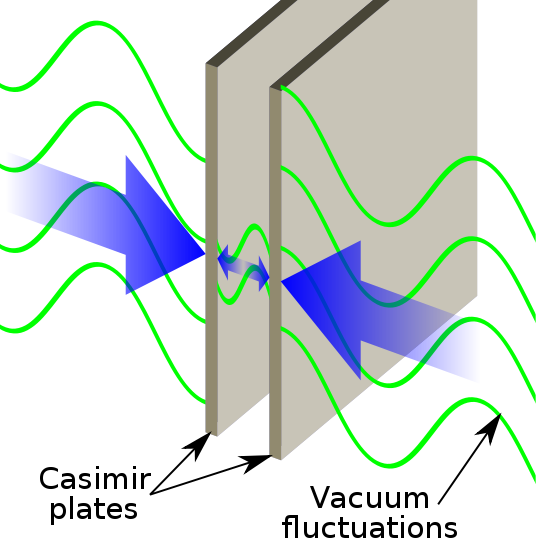
\includegraphics[scale=0.3]{casimir.png}
    \end{center}
}

\frame {
    \frametitle{Geometry plane--sphere}

    \begin{center}
    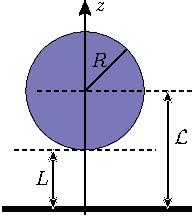
\includegraphics[scale=1.8]{geometry.pdf}
    \end{center}
}

\frame {
    \frametitle{Formulas...}

    \begin{itemize}
    \item Free Energy:
    \begin{equation}
    \nonumber
    \mathcal{F} = 2\kb T \, {\sum_{n=0}^\infty}^\prime {\sum_{m=0}^\infty}^\prime \log\det \left[ \mathbbm{1} - \mathcal{M}^{(m)}(\xi_n)\right]
    \end{equation}

    \item Matsubara-Frequencies:
    \begin{equation}
    \nonumber
    \xi_n = \frac{2\pi n \kb T}{\hbar}
    \end{equation}

    \item Round-Trip--Operator:
    \begin{equation}
    \nonumber
    \mathcal{M}^{(m)}(\xi_n) = \left(\begin{array}{cc}
    \nonumber
    \mathcal{M}^{(m)}(E,E) & \mathcal{M}^{(m)}(E,M) \\
    \nonumber
    \mathcal{M}^{(m)}(M,E) & \mathcal{M}^{(m)}(M,M)
    \end{array}
    \right)
    \end{equation}
    \end{itemize}
}

\frame {
    \frametitle{and even more formulas...}

    \begin{itemize}
    \item Matrix elements:
    \begin{align}
    \nonumber
    \mathcal{M}^{(m)}(E,E)_{\ell_1 \ell_2} &=  \Lambda^{(m)}_{\ell_1 \ell_2} a_{\ell_1} \left[ A^{(m)}_{\ell_1 \ell_2,\TE} + B^{(m)}_{\ell_1 \ell_2, \TM}\right] \\
    \nonumber
    \mathcal{M}^{(m)}(M,M)_{\ell_1 \ell_2} &=  \Lambda^{(m)}_{\ell_1 \ell_2} b_{\ell_1} \left[ A^{(m)}_{\ell_1 \ell_2,\TM} + B^{(m)}_{\ell_1 \ell_2, \TE}\right] \\
    \nonumber
    \mathcal{M}^{(m)}(E,M)_{\ell_1 \ell_2} &=  \Lambda^{(m)}_{\ell_1 \ell_2} a_{\ell_1} \left[ C^{(m)}_{\ell_1 \ell_2,\TE} + D^{(m)}_{\ell_1 \ell_2, \TM}\right] \\
    \nonumber
    \mathcal{M}^{(m)}(M,E)_{\ell_1 \ell_2} &= -\Lambda^{(m)}_{\ell_1 \ell_2} b_{\ell_1} \left[ C^{(m)}_{\ell_1 \ell_2,\TM} + D^{(m)}_{\ell_1 \ell_2, \TE}\right]
    \end{align}

    \item $a_\ell$, $b_\ell$: Mie-coefficients

    \item $\Lambda_{\ell_1 \ell_2}$ prefactor
    \begin{equation}
    \nonumber
    \Lambda_{\ell_1 \ell_2}^{(m)} = 
    -\sqrt{ \frac{(2\ell_1+1)\,(2\ell_2+1)\,(\ell_1-m)!\,(\ell_2-m)!}{(\ell_1+m)!\, (\ell_2+m)!\, \ell_1(\ell_1+1) \, \ell_2(\ell_2+1)} }
    \end{equation}
    \end{itemize}
}

\section{Unit tests}
\frame {
    \frametitle{Starting situation}

    The starting situation:
    \begin{itemize}
    \item you did the derivation
    \item you have a bunch of probably complicated formulas
    \item you can't solve the problem analytically
    \item you need code that solves your problem
    \end{itemize}

    \vfill

    From here:
    \begin{itemize}
    \item top to bottom
    \item bottom to top
    \end{itemize}

    \only<2> {
        \ \\
        \begin{center}
        Let's start bottom to top!
        \end{center}
    }
}

\begin{frame}[fragile]{Let's start with the prefactor!}
    \begin{equation}
    \nonumber
    \Lambda_{\ell_1 \ell_2}^{(m)} = 
    -\sqrt{ \frac{(2\ell_1+1)\,(2\ell_2+1)\,(\ell_1-m)!\,(\ell_2-m)!}{(\ell_1+m)!\, (\ell_2+m)!\, \ell_1(\ell_1+1) \, \ell_2(\ell_2+1)} }
    \end{equation}

    \vfill

    The code:
    \begin{lstlisting}
from __future__ import division
from math import sqrt, factorial as fac

def Lambda(l1,l2,m):
    num   = (2*l1+1)*(2*l2+1)*fac(l1-m)*fac(l2-m)
    denom = fac(l1+m)*fac(l2+m)*l1*(l1+1)*l2*(l2+1)
    return -sqrt(num/denom)
    \end{lstlisting}
\end{frame}

\begin{frame}{Testing}
    \begin{center}
    \huge So, what now?
    \end{center}
\end{frame}

\begin{frame}{Unit-Tests}
    Idea: At least one test for every function you write

    \vfill

    benefits:
    \begin{itemize}
        \item find problems early
        \item avoid regressions
        \item documentation
    \end{itemize}

    \vfill

    It's easy! There are modueles for almost every language!
\end{frame}

\begin{frame}[fragile]{The test}
\begin{lstlisting}
from __future__ import division
from casimir import *
import unittest

class CasimirTest(unittest.TestCase):
  def test_lambda(self):
    self.assertAlmostEqual(Lambda(1,1,0)/(-1.5), 1)
    self.assertAlmostEqual(Lambda(20,15,4)/(-1.18121789e-11), 1)
    self.assertAlmostEqual(Lambda(80,80,80)/(-5.26980602e-287), 1)

if __name__ == "__main__":
    unittest.main()
\end{lstlisting}
\end{frame}

\begin{frame}[fragile]{Output}
\scriptsize
\begin{verbatim}
F
======================================================================
FAIL: test_lambda (__main__.CasimirTest)
----------------------------------------------------------------------
Traceback (most recent call last):
  File "casimir_test.py", line 9, in test_lambda
    self.assertAlmostEqual(Lambda(80,80,80)/(-5.26980602e-287), 1)
AssertionError: 0.0 != 1 within 7 places

----------------------------------------------------------------------
Ran 1 test in 0.000s

FAILED (failures=1)
\end{verbatim}
\end{frame}

\begin{frame}{What went wrong?}
    \begin{equation}
    \nonumber
    \Lambda_{\ell_1 \ell_2}^{(m)} = 
    -\sqrt{ \frac{(2\ell_1+1)\,(2\ell_2+1)\,(\ell_1-m)!\,(\ell_2-m)!}{(\ell_1+m)!\, (\ell_2+m)!\, \ell_1(\ell_1+1) \, \ell_2(\ell_2+1)} }
    \end{equation}

    \vfill
    \begin{itemize}
        \item $n!$ becomes large
        \item numerator or denumerator may extend range of doubles
        \item \texttt{denom} $\approx 9.33 10^{576}$
        \item division cannot take place
    \end{itemize}

    \vfill
    Solution: Avoid division
\end{frame}

\begin{frame}{Solution}
    Use logarithms!

    \begin{align}
    \nonumber
    \Lambda_{\ell_1 \ell_2}^{(m)} &= 
    -\sqrt{ \frac{(2\ell_1+1)\,(2\ell_2+1)\,(\ell_1-m)!\,(\ell_2-m)!}{(\ell_1+m)!\, (\ell_2+m)!\, \ell_1(\ell_1+1) \, \ell_2(\ell_2+1)} } \\
    \nonumber
    &= \sqrt{\frac{(2\ell_1+1)\,(2\ell_2+1)}{\ell_1(\ell_1+1)\,\ell_2(\ell_2+1)}} \\
    \nonumber
    &\times \exp\left[{\frac{\log(\ell_1-m)!-\log(\ell_1+m)!+\dots}{2}}\right]
    \end{align}
\end{frame}
    
\begin{frame}[fragile]{The second try}
    Code:
    \begin{lstlisting}
def Lambda(l1,l2,m):
    return -sqrt( (2*l1+1)*(2*l2+1) / \
                  (l1*l2*(l1+1)*(l2+1)) ) \
      * exp( (lgamma(l1-m+1)+lgamma(l2-m+1)\
             -lgamma(l1+m+1)-lgamma(l2+m+1))/2 )
    \end{lstlisting}

    \only<2> {
        \begin{center}
        And the test works!
        \end{center}
        }
\end{frame}

\begin{frame}{Let's pause for a moment!}
    \begin{itemize}
        \item numerical code can be tricky
        \item ...especially floating point arithmetics 
        \item unit tests can help finding bugs!
        \item unit tests can help preventing bugs!
        \vfill
        \item you can test a function...
        \item or your whole program
    \end{itemize}

    \vfill
    \hfill
    
\includegraphics[scale=0.3]{bug.png}
\end{frame}

\begin{frame}[fragile]{The test}
\begin{lstlisting}
from Casimir import PerfectReflectors
import unittest

class CasimirTest(unittest.TestCase):
  def test_casimir(self):
    ScriptL = 2e-6
    R = 1e-6
    T = 50
    Fexp = 2.95192899663732e-22
    lmax = 10
    nmax = 100
    casimir = PerfectReflectors(R,ScriptL,T,lmax=lmax)
    Fcalc = casimir.F(nmax=nmax)
    self.assertAlmostEqual(Fexp/Fcalc, 1)

if __name__ == "__main__":
    unittest.main()
\end{lstlisting}
\end{frame}

\section{Revision control systems}
\begin{frame}{Revision control systems}
\begin{itemize}
    \item example: Wikipedia editions
    \item you can commit changes
    \item you can collaborate
    \item you can see the differences between versions
    \item you can see the difference between the last (commited) version and your current code
    \item it is also kind of a backup
    \item it will document your work
    \item it will save you time!
    \item examples: git or subversion
\end{itemize}
\end{frame}

\begin{frame}{Example}

\begin{itemize}
\item you spend hours rewriting your code
\item now it doesn't work anymore
\item use a diff
\end{itemize}

\vfill

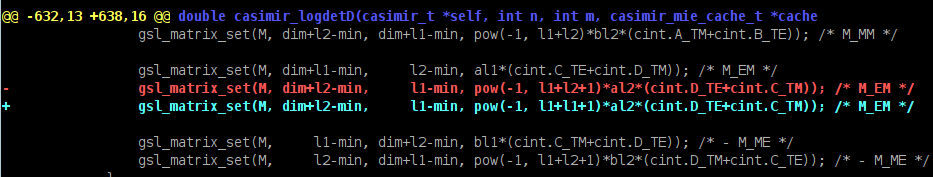
\includegraphics[scale=0.5]{svn.png}
\end{frame}

\section{Optimization}

\begin{frame}{Optimization}
\huge
\begin{center}
My code is running too slow? What can I do?
\end{center}
\end{frame}

\begin{frame}{Optimization}
\begin{itemize}
    \item don't optimize at an early stage!
    \item use a profiler and find why your program is slow
    \item use a better algorithm
    \item do you have to calculate everything?
    \item do you calculate things to often?
    \item exploit symmetries
    \item use caches
    \item if C: use optimization, inlines and macros
\end{itemize}
\end{frame}

\begin{frame}{Example}
What about $A$, $B$, $C$ and $D$?

\begin{align}
\nonumber
A_{\ell_1 \ell_2,p}^{(m)}(\xi) &= \frac{m^2 \xi}{\c} \int_0^\infty \mathrm{d}k \, \frac{1}{k \kappa} \, r_p \, \e^{-2\kappa\mathcal{L}} \, \Plm{\ell_1}{m}\left(\frac{\kappa\c}{\xi}\right) \Plm{\ell_2}{m}\left(-\frac{\kappa\c}{\xi}\right) \\
\nonumber
B_{\ell_1 \ell_2,p}^{(m)}(\xi) &= \frac{\c^3}{\xi^3} \int_0^\infty \mathrm{d}k \, \frac{k^3}{\kappa} \, r_p \, \e^{-2\kappa\mathcal{L}} \, \Plm{\ell_1}{m}^\prime\left(\frac{\kappa\c}{\xi}\right) \Plm{\ell_2}{m}^\prime\left(-\frac{\kappa\c}{\xi}\right) \\
\nonumber
C_{\ell_1 \ell_2,p}^{(m)}(\xi) &= -\frac{\imag m\c}{\xi} \int_0^\infty \mathrm{d}k \, \frac{k}{\kappa} \, r_p \, \e^{-2\kappa\mathcal{L}} \, \Plm{\ell_1}{m}\left(\frac{\kappa\c}{\xi}\right) \Plm{\ell_2}{m}^\prime\left(-\frac{\kappa\c}{\xi}\right) \\
\nonumber
D_{\ell_1 \ell_2,p}^{(m)}(\xi) &= -\frac{\imag m\c}{\xi} \int_0^\infty \mathrm{d}k \, \frac{k}{\kappa} \, r_p \, \e^{-2\kappa\mathcal{L}} \, \Plm{\ell_1}{m}^\prime\left(\frac{\kappa\c}{\xi}\right) \Plm{\ell_2}{m}\left(-\frac{\kappa\c}{\xi}\right)
\end{align}

\begin{equation}
\nonumber
\kappa = \sqrt{\frac{\xi^2}{\c^2}+k^2}
\end{equation}
\end{frame}

\begin{frame}{Example}
    \begin{itemize}
        \item my first approach: Use integration of scipy module
        \item my first result: Horrible slow, integration often doesn't converge 
        \item solution: investigate properties of integral
    \end{itemize}
\end{frame}

\begin{frame}{Example}
After substituation:
\begin{align}
\nonumber
A_{\ell_1 \ell_2}^{(m)} &= A_0 \int_0^\infty \mathrm{d}x \, \frac{\e^{-x}}{x^2+2\tilde\xi x} \Plm{\ell_1}{m}\left( 1+\frac{x}{\tilde\xi} \right) \Plm{\ell_2}{m}\left( 1+\frac{x}{\tilde\xi} \right) \\
\nonumber
B_{\ell_1 \ell_2}^{(m)} &= B_0 \int_0^\infty \mathrm{d}x \, \left(x^2+2\tilde\xi x\right) \e^{-x} \Plm{\ell_1}{m}^\prime\left( 1+\frac{x}{\tilde\xi} \right) \Plm{\ell_2}{m}^\prime\left( 1+\frac{x}{\tilde\xi} \right) \\
\nonumber
C_{\ell_1 \ell_2}^{(m)} &= C_0 \int_0^\infty \mathrm{d}x \, \e^{-x} \, \Plm{\ell_1}{m}\left( 1+\frac{x}{\tilde\xi} \right) \Plm{\ell_2}{m}^\prime\left( 1+\frac{x}{\tilde\xi} \right) \\
\nonumber
D_{\ell_1 \ell_2}^{(m)} &= D_0 \int_0^\infty \mathrm{d}x \, \e^{-x} \, {\Plm{\ell_1}{m}}^\prime\left( 1+\frac{x}{\tilde\xi} \right) \Plm{\ell_2}{m}\left( 1+\frac{x}{\tilde\xi} \right)
\end{align}

\begin{equation}
\nonumber
\tilde\xi = 2\mathcal{L}\frac{\xi}{\c}
\end{equation}
\end{frame}

\begin{frame}{Example}
\begin{itemize}
    \item integrands are of the form $f(x) e^{-x}$, where $f(x)$ is a polynomial
    \item use Gauss-Laguerre: $\int_0^\infty \e^{-x} f(x) \approx \sum_i w_i f(x_i)$
    \item error $\propto f^{(2n)}(x)$
    \item if $A$, $B$, $C$, $D$ are calculated as a vector: one must only compute associated legendre polynomial once
    \item there are symmetries between $A$ and $B$, $C$ and $D$
    \item Better algorithm:\\ program runs way faster, results are exact (within double precision)
\end{itemize}
\end{frame}

\begin{frame}{Example II}
    \begin{itemize}
    \item Free Energy:
    \begin{equation}
    \nonumber
    \mathcal{F} = 2\kb T \, {\sum_{n=0}^{n_\text{max}}}^\prime {\sum_{m=0}^{l_\text{max}}}^\prime \log\det \left[ \mathbbm{1} - \mathcal{M}^{(m)}(\xi_n)\right]
    \end{equation}
    \item summands may be small when $m$ increases
    \item one may crop summation over $m$
    \end{itemize}
\end{frame}

\begin{frame}[fragile]{Profiler: gprof}
\begin{itemize}
    \item compile with flag \texttt{-pg}
    \item run program
    \item gprof program
\end{itemize}
\tiny
\begin{verbatim}
Each sample counts as 0.01 seconds.
  %   cumulative   self              self     total
 time   seconds   seconds    calls  ms/call  ms/call  name
 67.80      1.64     1.64  5801418     0.00     0.00  _plm_array
 14.88      2.00     0.36  5801418     0.00     0.00  plm_Yl12md
 12.82      2.31     0.31  5801418     0.00     0.00  casimir_integrands_vec
  2.48      2.37     0.06   254646     0.00     0.01  gausslaguerre_integrate_vec
  0.83      2.39     0.02  5801418     0.00     0.00  casimir_rTM
  0.83      2.41     0.02      817     0.02     2.95  casimir_logdetD
  0.41      2.42     0.01                             plm_dPlm
  0.00      2.42     0.00   254646     0.00     0.01  casimir_integrate
  0.00      2.42     0.00    27349     0.00     0.00  casimir_Xi
  0.00      2.42     0.00      878     0.00     0.00  casimir_logdet1m
  0.00      2.42     0.00      878     0.00     0.00  la_norm_froebenius
  0.00      2.42     0.00      878     0.00     0.00  logdet1m_eigenvalues
  0.00      2.42     0.00       19     0.00     0.00  casimir_mie_cache_alloc
\end{verbatim}
\end{frame}

\section{Bits and pieces}
\subsection{Reproducability}
\begin{frame}{Reproducability}
\begin{itemize}
\item what were the parameters given?
\item what version of the code were you using?
\item what changes?
\item when?
\item on which machine?
\item append data to plots
\end{itemize}
\end{frame}

\subsection{Style}
\begin{frame}{Watch your style!}
    \begin{itemize}
        \item Use indention
        \item Use meaningful names for your variables
        \item Use comments
        \item Use functions/modules
        \item Be lazy when you can
        \item Be hardworking when you must
    \end{itemize}
\end{frame}

\subsection{C and gcc}
\begin{frame}{When programming C and gcc}
\begin{itemize}
    \item enable warnings \texttt{-Wall} 
    \item consider warnings to be errors \texttt{-Werror}
    \item use optimization: \texttt{-O2} or \texttt{-O3} or \texttt{-O4}
    \item put debugging symbols in the executable \texttt{-g}
    \item use functions and mark them as inlines -- if necessary
    \item use the preprocessor and makros
    \item if you need portability: \texttt{-pedantic}, \texttt{-ansi} and (if necessary) \texttt{-Dinline=}
    \item you may use a debugger: gdb
\end{itemize}
\end{frame}

\begin{frame}
\huge
\begin{center}
Thank you for your attention! :)
\end{center}
\end{frame}


\end{document}
